\documentclass[12pt,AutoFakeBold]{article}%第二个参数解决宋体没有粗体的问题
\usepackage{booktabs}%绘制三线表
\usepackage{fontspec}%控制字体
\usepackage[version=3]{mhchem}%化学反应式
\usepackage{xeCJK}%控制中文字体
\usepackage{latexsym}%绘制特殊数学符号
\usepackage[a4paper]{geometry}%纸张大小和页边距
\usepackage{pdfpages}%插入pdf页面
\usepackage{titlesec}%控制标题格
\usepackage{graphicx, epstopdf}%此处使.eps文件可转化成.pdf并应用自动编号功能
\usepackage[journal=angew]{chemstyle}%此处设置图式的样式
\usepackage{siunitx}%数学模式中使用SI单位
\usepackage{color}%提供颜色支持
\usepackage{listings,xcolor}
\usepackage{amsfonts}
\usepackage{indentfirst}

\geometry{left=2.5cm,right=2.5cm,top=2.5cm,bottom=2.5cm}%页边距设置
\setmainfont{Times New Roman}%英文字体
\setCJKmainfont{SimSun}%中文字体
\newfontfamily\arial{Arial}%Arial字体
\XeTeXlinebreaklocale "zh"%中文自动换行
\XeTeXlinebreakskip = 0pt plus 1pt%中文自动换行

\lstset{
numbers=left,
framexleftmargin=10mm,
frame=none,
backgroundcolor=\color[RGB]{245,245,244},
keywordstyle=\bf\color{blue},
identifierstyle=\bf,
numberstyle=\color[RGB]{0,192,192},
commentstyle=\it\color[RGB]{0,96,96},
stringstyle=\rmfamily\slshape\color[RGB]{128,0,0},
showstringspaces=false
}

\newcommand{\dif}{\mathrm{d}}

\begin{document}
    % cover
    \vspace*{4cm}
    \begin{center}
        \Huge{\textbf{高压油管压力控制的数学模型}}
    \end{center}
    \vspace*{5cm}
    \rule{\textwidth}{1mm}
    \large{    
    \textbf{摘要}\quad 对高压油管中的燃油注入和喷出的数学模型的建立,是研究和改善燃油发动机工作状况的必要前提。在本问题中,我们考察了一个由高压油泵、高压油管、喷油嘴和减压阀等部件组成的简单高压油路系统。我们将复杂的高压油路系统建立成一个形式简单而统一的数学形式
    \[\frac{\dif p}{E\dif t}=\frac{Q_{in}-Q_{out}}{V}\]
    并从这个简洁优美的式子,推导出关于这个高压油路的控制理论依据。\\
    \textbf{关键词}\quad 高压油管\quad 压力控制\quad 数学模型\\
    }
    \rule{\textwidth}{1mm}
    \newpage
    % main body
    \section{问题重述与分析}
    对高压油管中的燃油注入和喷出的数学模型的建立,是研究和改善燃油发动机工作状况的必要前提。在本问题中,我们考察了一个由高压油泵、高压油管、喷油嘴和减压阀等部件组成的简单高压油路系统。\par
    我们首先考虑了这个高压油路系统最简单的情况,即油泵可以稳定注入恒压的高压油,喷嘴以简单函数方式喷出油料;随后,我们把高压油泵的实际工作情况考虑进来,同时考虑了喷油嘴工作的本质,模型变得复杂起来;最后,我们考虑了实践中常见的多喷嘴油路的工作情况,并引入减压阀来控制高压油管内部的压力变化。问题不断复杂化,并不断接近高压油路的真实工作状态,实用性不断提高。\par

    \section{模型设计与计算}
    \subsection{基本模型设计}
    我们的目标是解出高压油管内部压力$p$与时间$t$的关系,记作
    \begin{equation}
        p=p(t)
    \end{equation}
    \par
    由条件可见,高压油管的内部体积$V$不变,由$\rho=\frac{m}{V}$可见,对高压油管内燃油密度造成影响的仅有高压油管内的燃油质量,用微分方程来表达就是
    \begin{equation}
        \dif\rho=\dif\left(\frac{m}{V}\right)=\frac{\dif m}{V}
        \label{eq1}
    \end{equation}
    \par
    首先我们考虑$\dif\rho$和$p$的关系。\par
    根据注1给出的条件,燃油的压力与其密度具有正相关关系,其关系可以用微分方程
    \begin{equation}
         \begin{cases}
            &\dif p=\frac{E}{\rho}\dif\rho\\
            &p_0=\SI{100}{\MPa},\rho_0=\SI{0.850}{\mg\per\cubic\mm}\\
            &E=E(p)
        \end{cases}
        \label{pandrho}
    \end{equation}
    描述,其中$E(p)$由附件3的数据给出,对附件3的数据用MATLAB作图并拟合得到方程,如图\ref{data3}
    \begin{equation}
        E(p)=0.0001p^3-0.001082p^2+5.474p+1532\ \ \ \ (r^2=1.0000)
    \end{equation}
    \begin{figure}[H]
        \centering
        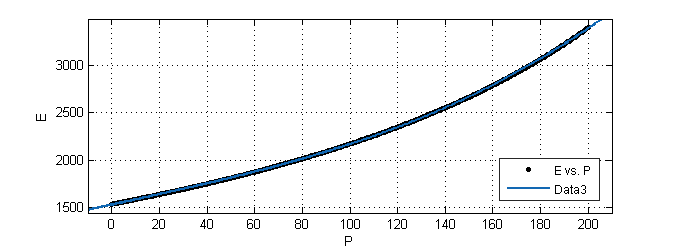
\includegraphics[scale=0.8]{figure/data3.png}
        \caption{燃油弹性模量$E$与压力$p$的非线性拟合结果}
        \label{data3}
    \end{figure}
    由以上的方程我们可以解出关系
    \begin{equation}
        \rho(p)=0.850e^{\int^p_{100}\frac{\dif p}{E(p)}}
        \label{eq2}
    \end{equation}
    \par
    其次,我们再来考虑$\dif m$和$p$与$t$的关系。\par
    $\dif m$由进入和喷出两部分组成。喷出部分对$\dif m$的贡献是时间的函数。单位时间喷出的油量(体积)用函数$Q_{out}(t)$表示,它的解析式在各个小题中有所不同,并且分段可微,所以喷出端造成的$\dif m$可以表述成
    \begin{equation}
        \dif m_{out}=-\rho Q_{out}(t)\dif t
        \label{eq3}
    \end{equation}\par
    进入部分对$\dif m$的贡献也是时间的函数。这个函数含有参数$T$,在上面提及过,它描述了单向阀的开启时间。单位时间进入的油量(体积)用函数$Q_{in}(t)$表示,它的解析式在各个小题中也有所不同,并且分段可微,所以喷出端造成的$\dif m$可以表述成
    \begin{equation}
        \dif m_{in}=\rho Q_{in}(t)\dif t
        \label{eq4}
    \end{equation}\par
    综上,联立方程\ref{eq1}、\ref{eq2}、\ref{eq3}、\ref{eq4},我们可以列出方程
    \begin{equation}
        \frac{\dif p}{E\dif t}=\frac{Q_{in}-Q_{out}}{V}
        \label{maineq}
    \end{equation}\par
    方程\ref{maineq}就是我们对本题建立的基本数学模型。接下来的部分中,我们将根据$Q_{in}(t)$和$Q_{out}(t)$的具体形式,对整个体系最佳$T$值的选择进行讨论。
    
    \subsection{问题1}
    在问题1中$Q_{out}(t)$的形式比较简单,它是由题目中图\ref{inputof1}给出的
    \begin{figure}[H]
        \centering
        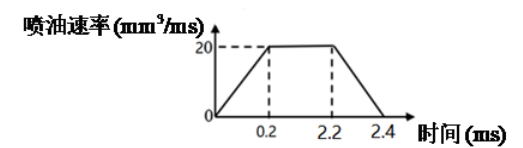
\includegraphics[scale=0.75]{figure/inputof1.png}
        \caption{问题1中的喷油速率}
        \label{inputof1}
    \end{figure}
    写成函数为
    \begin{equation}
        Q_{out}(t)=
        \begin{cases}
            100(t-100k)&100k\leq t\leq 100k+0.2,k\in\mathbb{N}\\
            20&100k+0.2\leq t\leq 100k+2.2,k\in\mathbb{N}\\
            -100(t-100k)+240&100k+2.2\leq t\leq 100k+2.4,k\in\mathbb{N}\\
        \end{cases}
    \end{equation}\par
    在问题1中$Q_{in}(t)$的形式也比较简单,它包括一个参数$T$,描述力单向阀每次开启的时长。我们定义$0-1$变量$\lambda=\lambda(t)$来描述供油处入口的截面积,它的形式为
    \begin{equation}
        \lambda=
        \begin{cases}
            1 & k(T+10)\leq t\leq k(T+10)+T,k\in\mathbb{N}\\
            0 & k(T+10)+T\leq t\leq (k+1)(T+10),k\in\mathbb{N}
        \end{cases}
    \end{equation}
    代入题目中给出的流量公式可得
    \begin{equation}
        Q_{in}(t)=\lambda CA\sqrt{\frac{2(p_h-p)}{\rho_h}}
    \end{equation}\par
    将$Q_{in}(t)$和$Q_{out}(t)$的具体形式代入方程\ref{maineq},发现所得方程是一阶常微分方程,所以尝试用差分法通过计算机进行数值解微分方程,取$\Delta t=\SI{0.01}{ms}$,用C++程序进行计算并用Python绘制出对应于不同$T$取值$p-t$变化图,以及差分过程中选用不同$\Delta t$对结果的影响,发现两条曲线非常接近,可以认为结果收敛可靠,如图\ref{ptfigure1}
    \begin{equation}
        \frac{p_{i+1}-p_i}{E(p_i)\Delta t}=\frac{1}{V_0}\left(\lambda CA\sqrt{\frac{2\left(p_h-p_i\right)}{\rho_h}}-Q_{out}(t_i)\right)
    \end{equation}
    \begin{figure}[H]
        \centering
        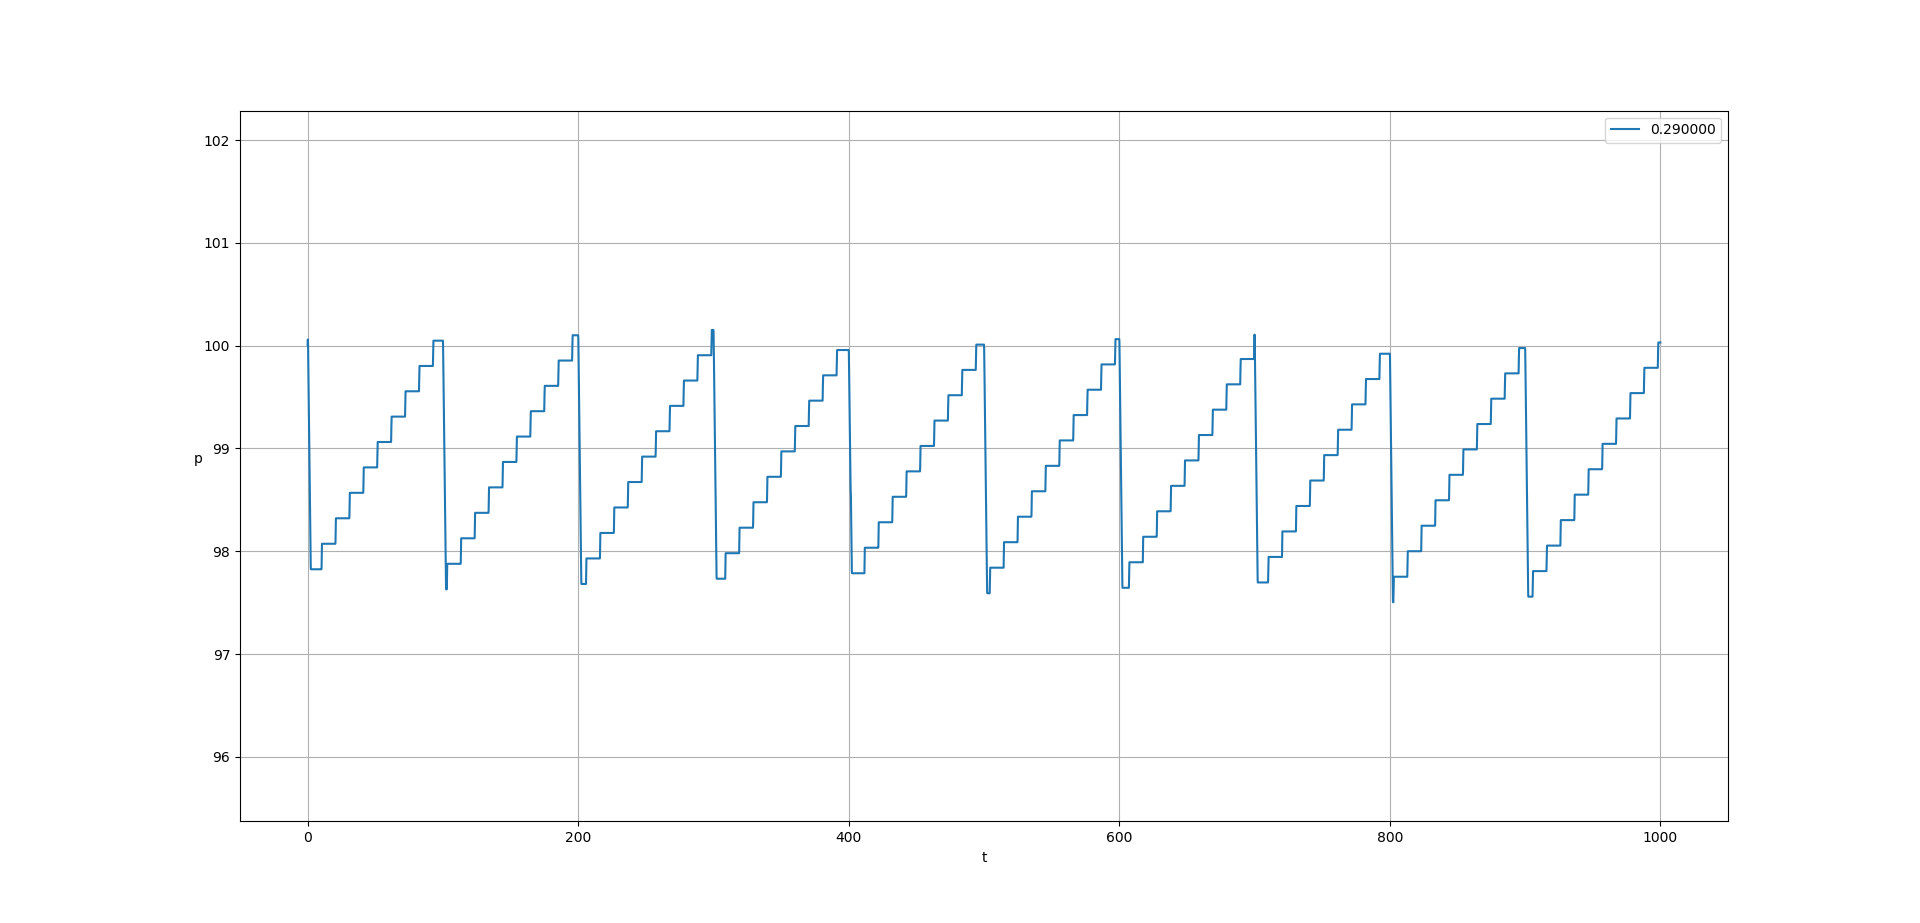
\includegraphics[scale=0.32]{figure/11-0.png}
        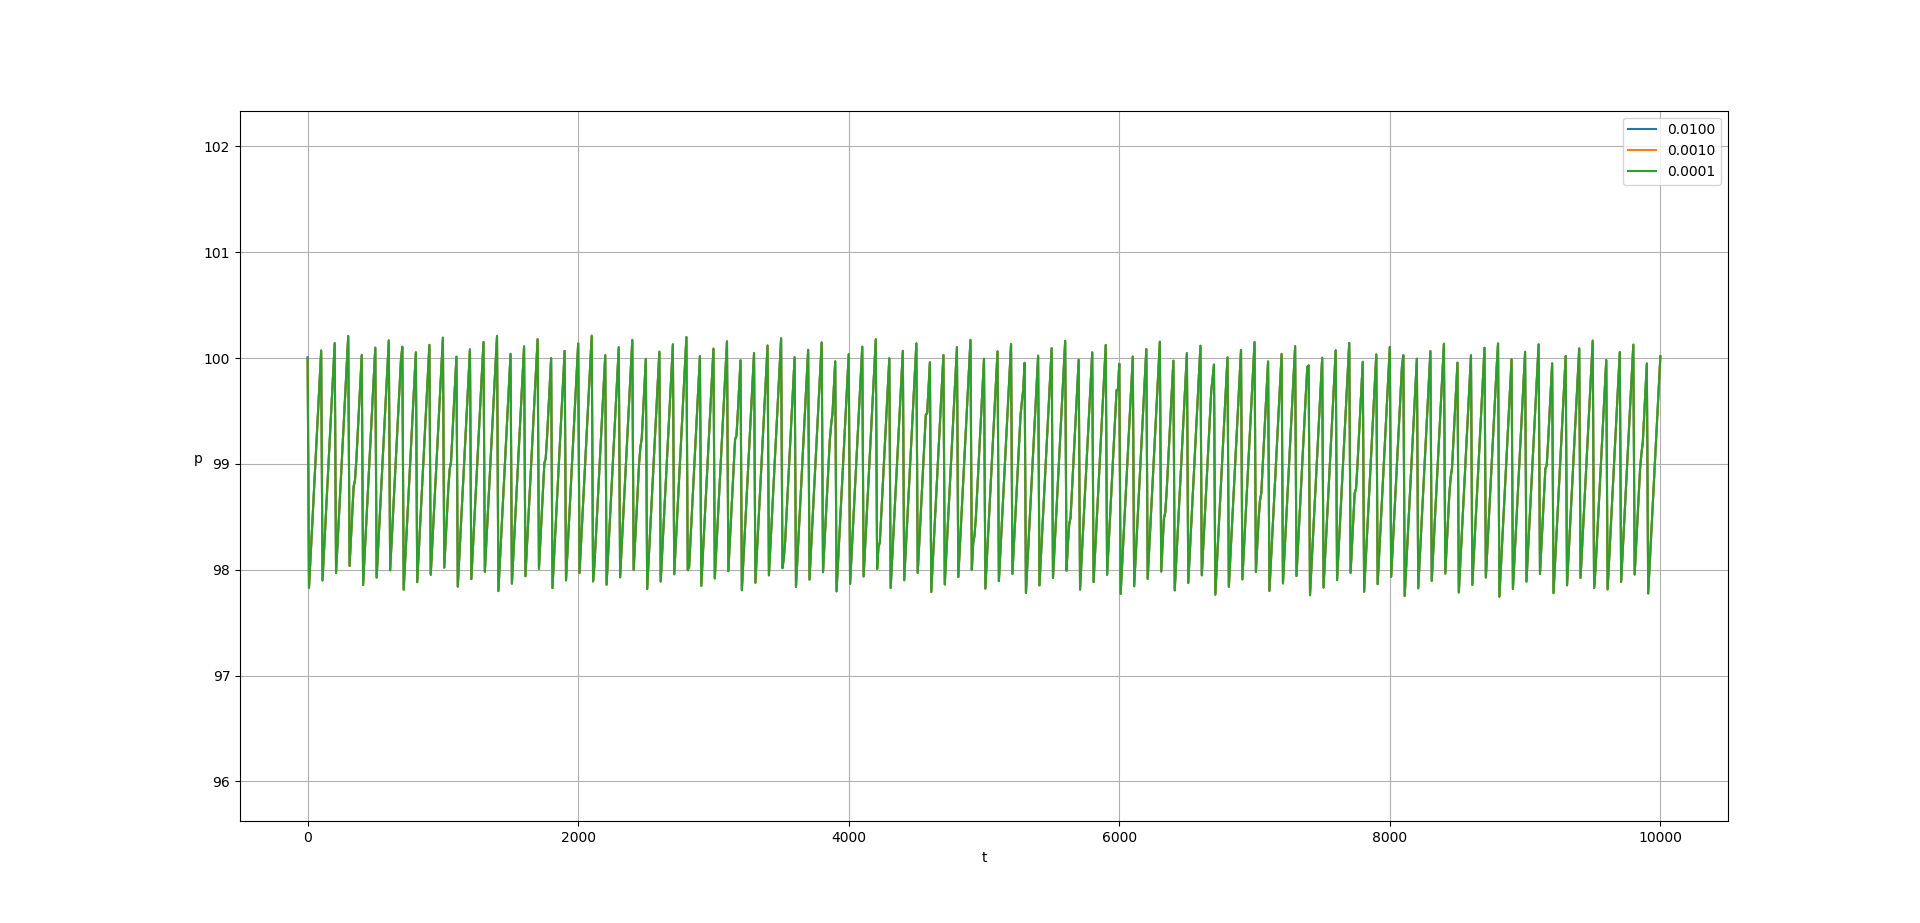
\includegraphics[scale=0.32]{figure/11-exgap-1}
        \caption{差分方程数值模拟结果}
        \label{ptfigure1}
    \end{figure}
    我们使用二分法对一定范围内的$T$进行搜索,用经过一定时间段后高压油管内油压力的变化$\Delta p$来评价“压力稳定在\SI{100}{\MPa}”的好坏,搜索出使压力变化最小时的单向阀开启时长$T=\SI{0.29}{\ms}$。\par
    同时,在数值模拟的过程中我们发现,只要$T$处于一定的范围内,在经过较长时间后,高压油管内的压力$p$都可以稳定地收敛到一个区间内,如图\ref{11top2},它描述了取不同的$T$值之后\SI{200000}{\ms}内高压油管内压力的变化趋势和范围。利用数值模拟可以求出这个区间大致为$[0.292,0.298]\si{\ms}$。\par
    \begin{figure}[H]
        \centering
        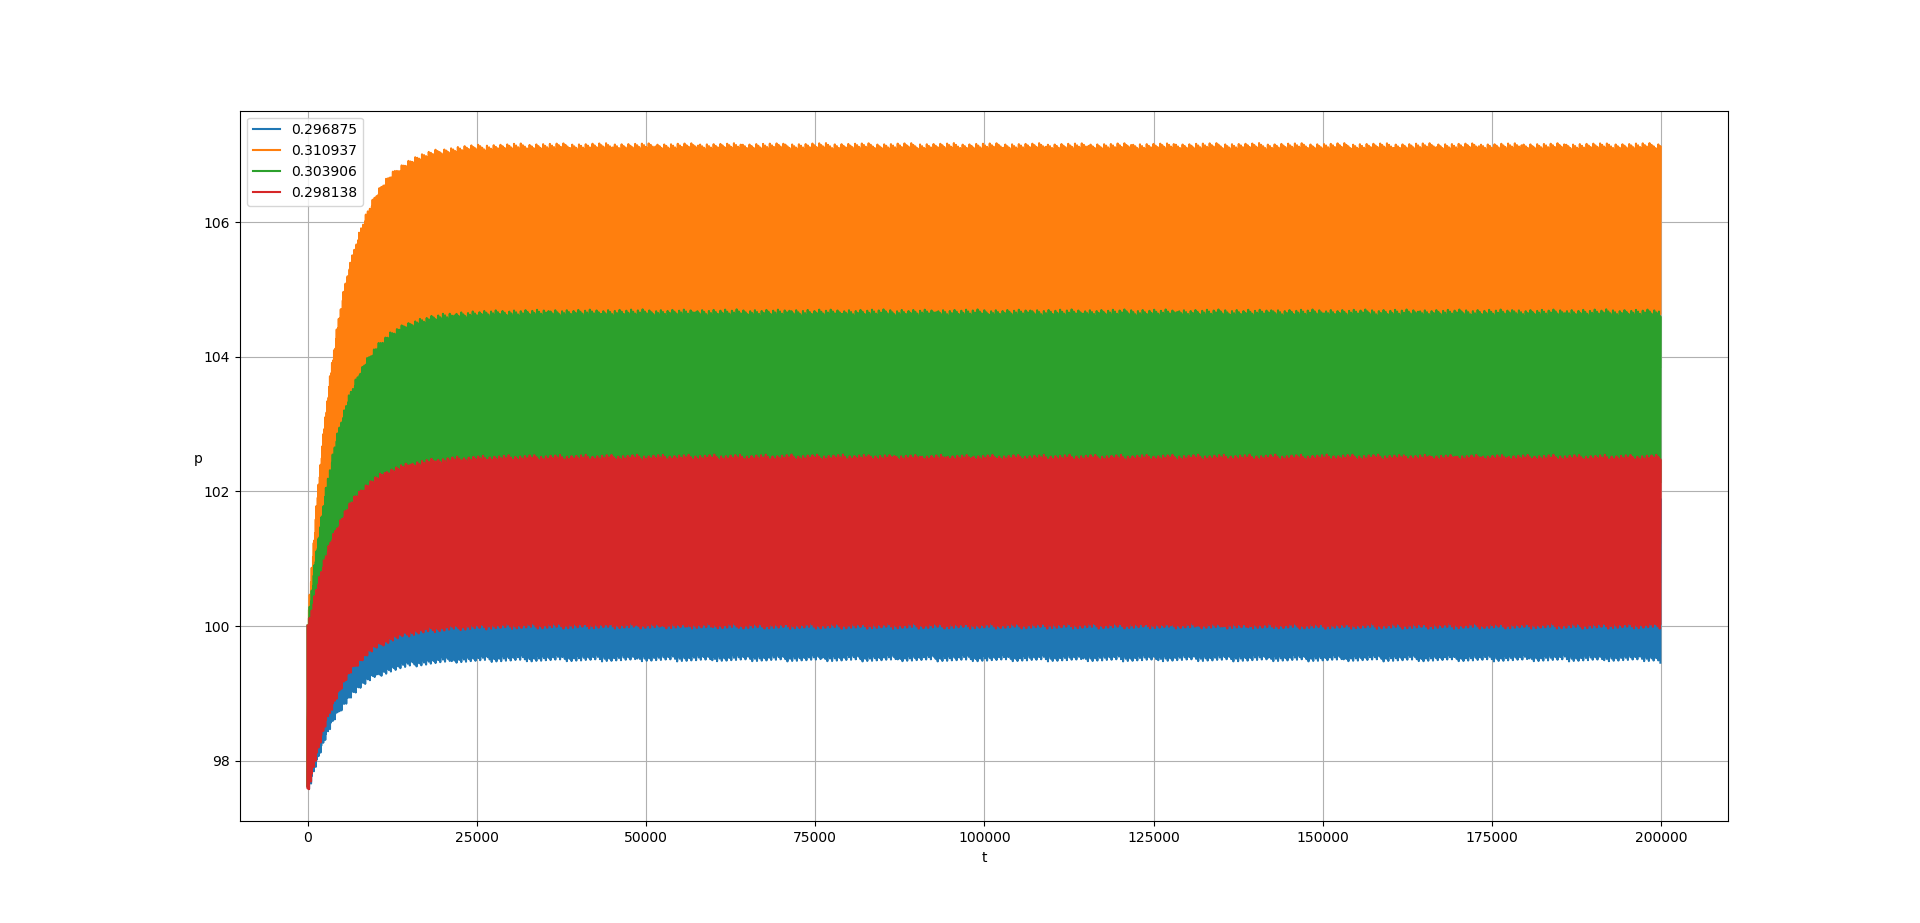
\includegraphics[scale=0.32]{figure/11-t-2.png}
        % 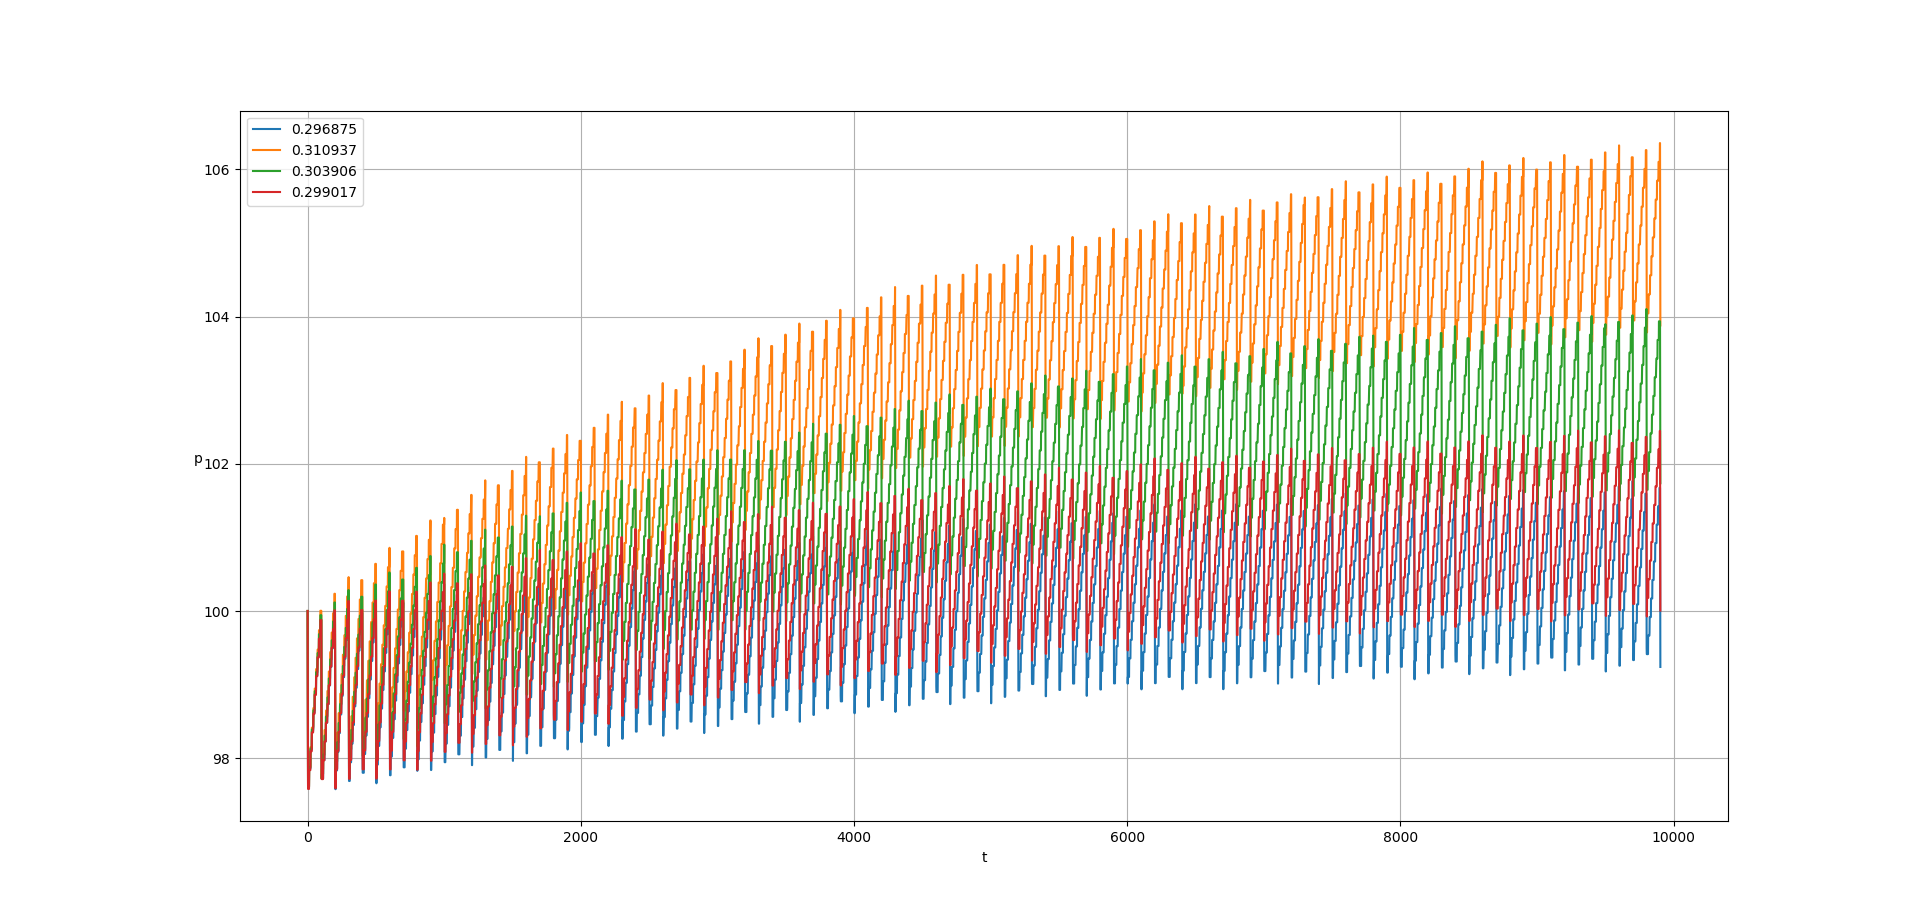
\includegraphics[scale=0.32]{figure/11-t-1.png}
        \caption{\SI{200000}{\ms}内不同喷油间隔值下高压油管压力与时间的关系}
        \label{11top2}
    \end{figure}
    同时,在前面的计算中我们只考虑了$t=0$时刻同时开始喷油和开始供油的情况,实际问题中,供油周期和喷油周期可能存在着相位差,但是通过数值模拟发现相位差造成的影响很小,在较长时间段内可以忽略,如图\ref{11exxwc}。\par
    \begin{figure}[H]
        \centering
        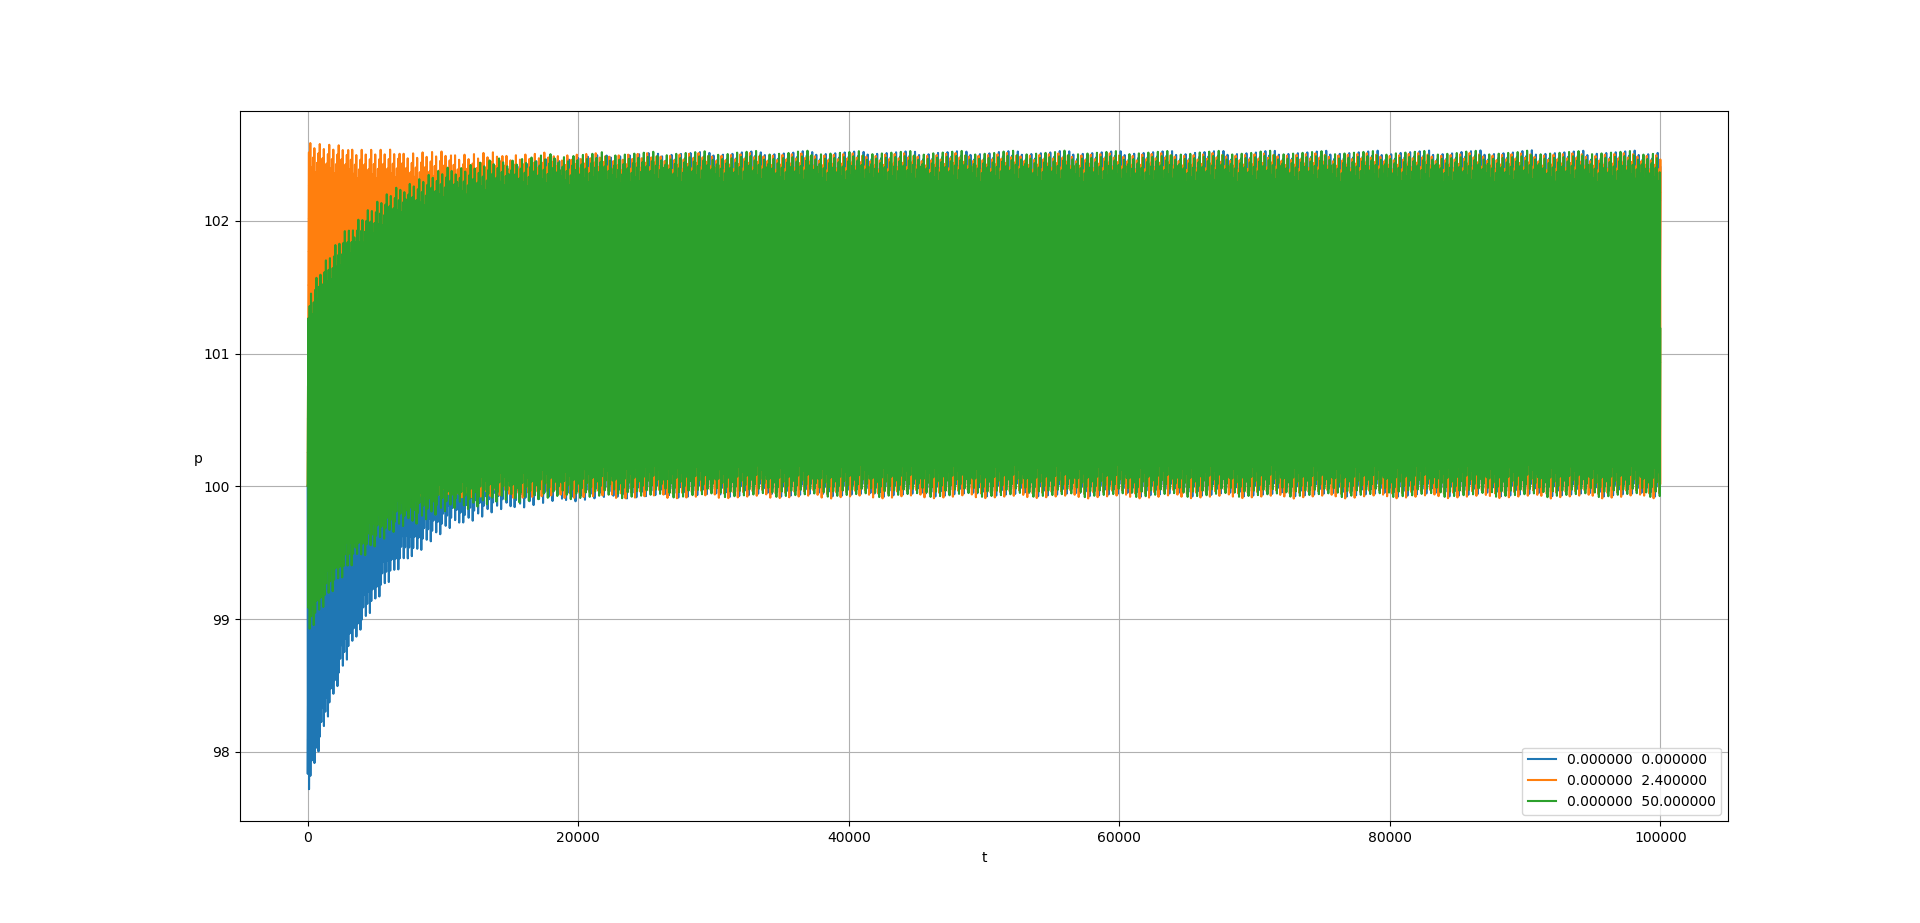
\includegraphics[scale=0.32]{figure/11-exxwc.png}
        \caption{相位差对$p-t$关系的影响}
        \label{11exxwc}
    \end{figure}
    对于将油管内的压力从\SI{100}{\MPa}提高到\SI{150}{\MPa}的情况,我们可以用同样的差分方程,分别模拟起始压力与\SI{2}{\s}、\SI{5}{\s}和\SI{10}{\s}后的压力差别为\SI{50}{\MPa}时的情况,同样通过二分法可以找出最佳的精确到百分位的单向阀开启时长$T_{2s}=\SI{0.89}{\ms}$、$T_{5s}=\SI{0.71}{\ms}$和$T_{10s}=\SI{0.70}{\ms}$。\par
    \begin{figure}[H]
        \centering
        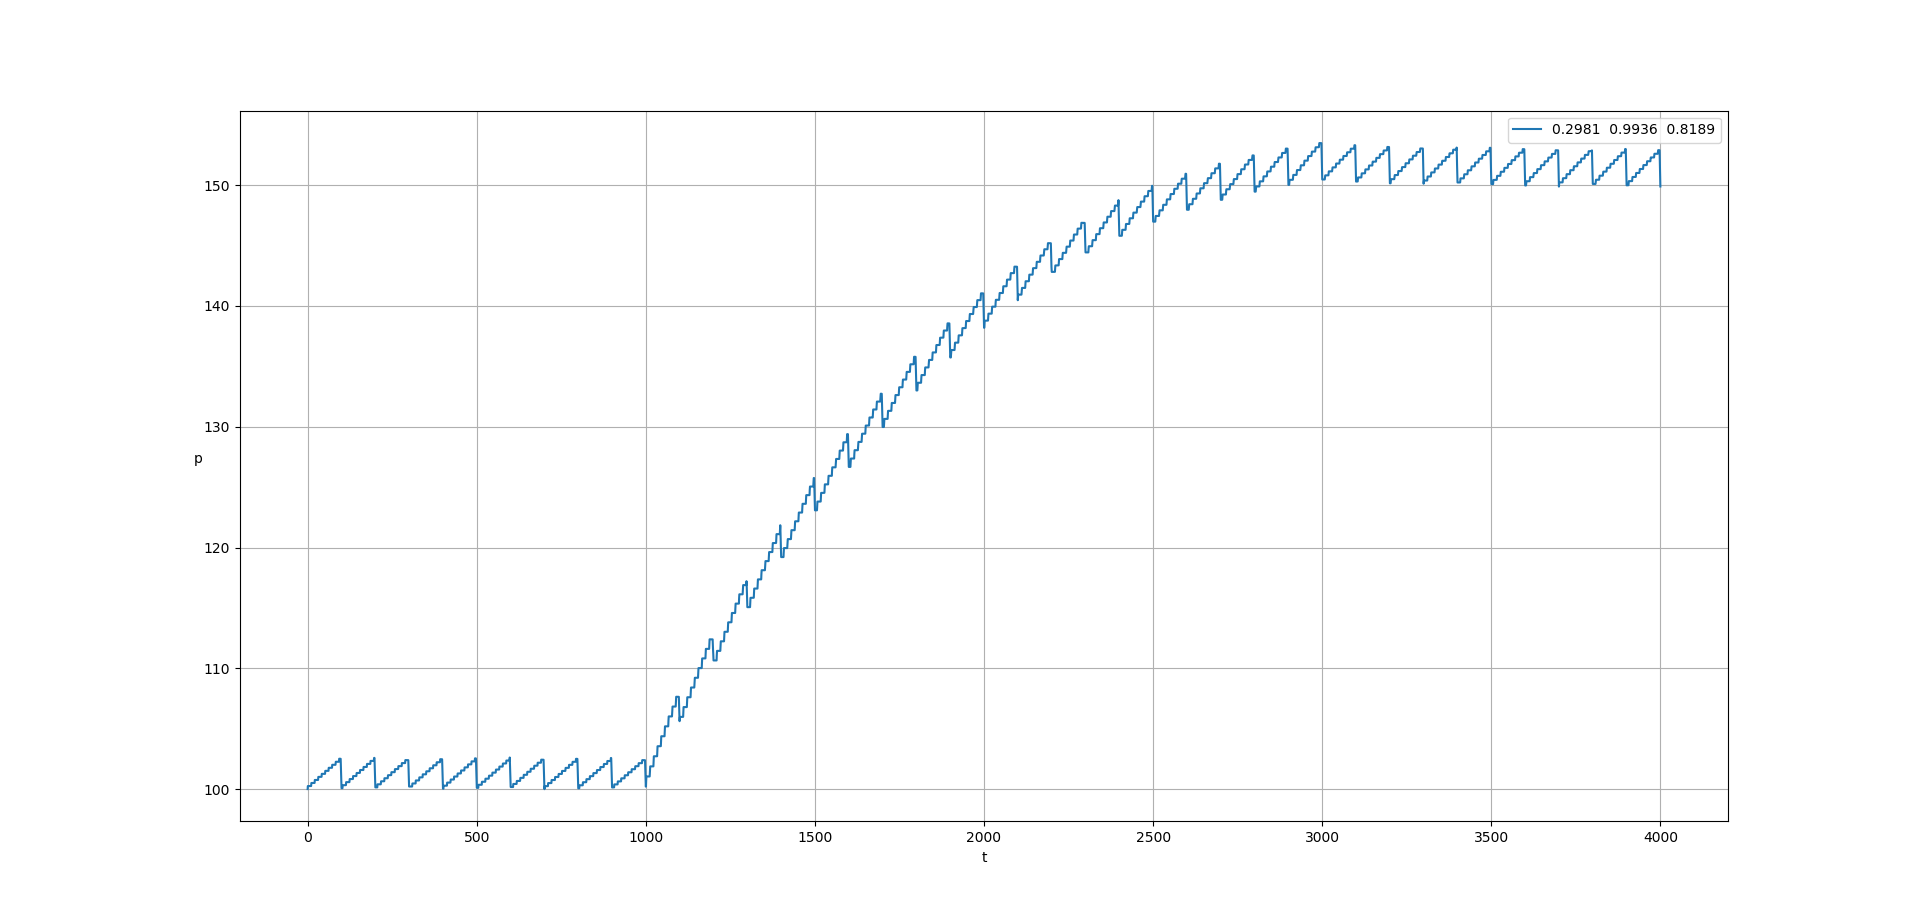
\includegraphics[scale=0.32]{figure/13-1-t.png}
        \caption{调整过程中的压力周期变化}
        \label{adjustpress}
    \end{figure}
    图\ref{12exxwc}描述了相位差对调整过程的影响,在调节完成后依旧可以收敛。\par
    \begin{figure}[H]
        \centering
        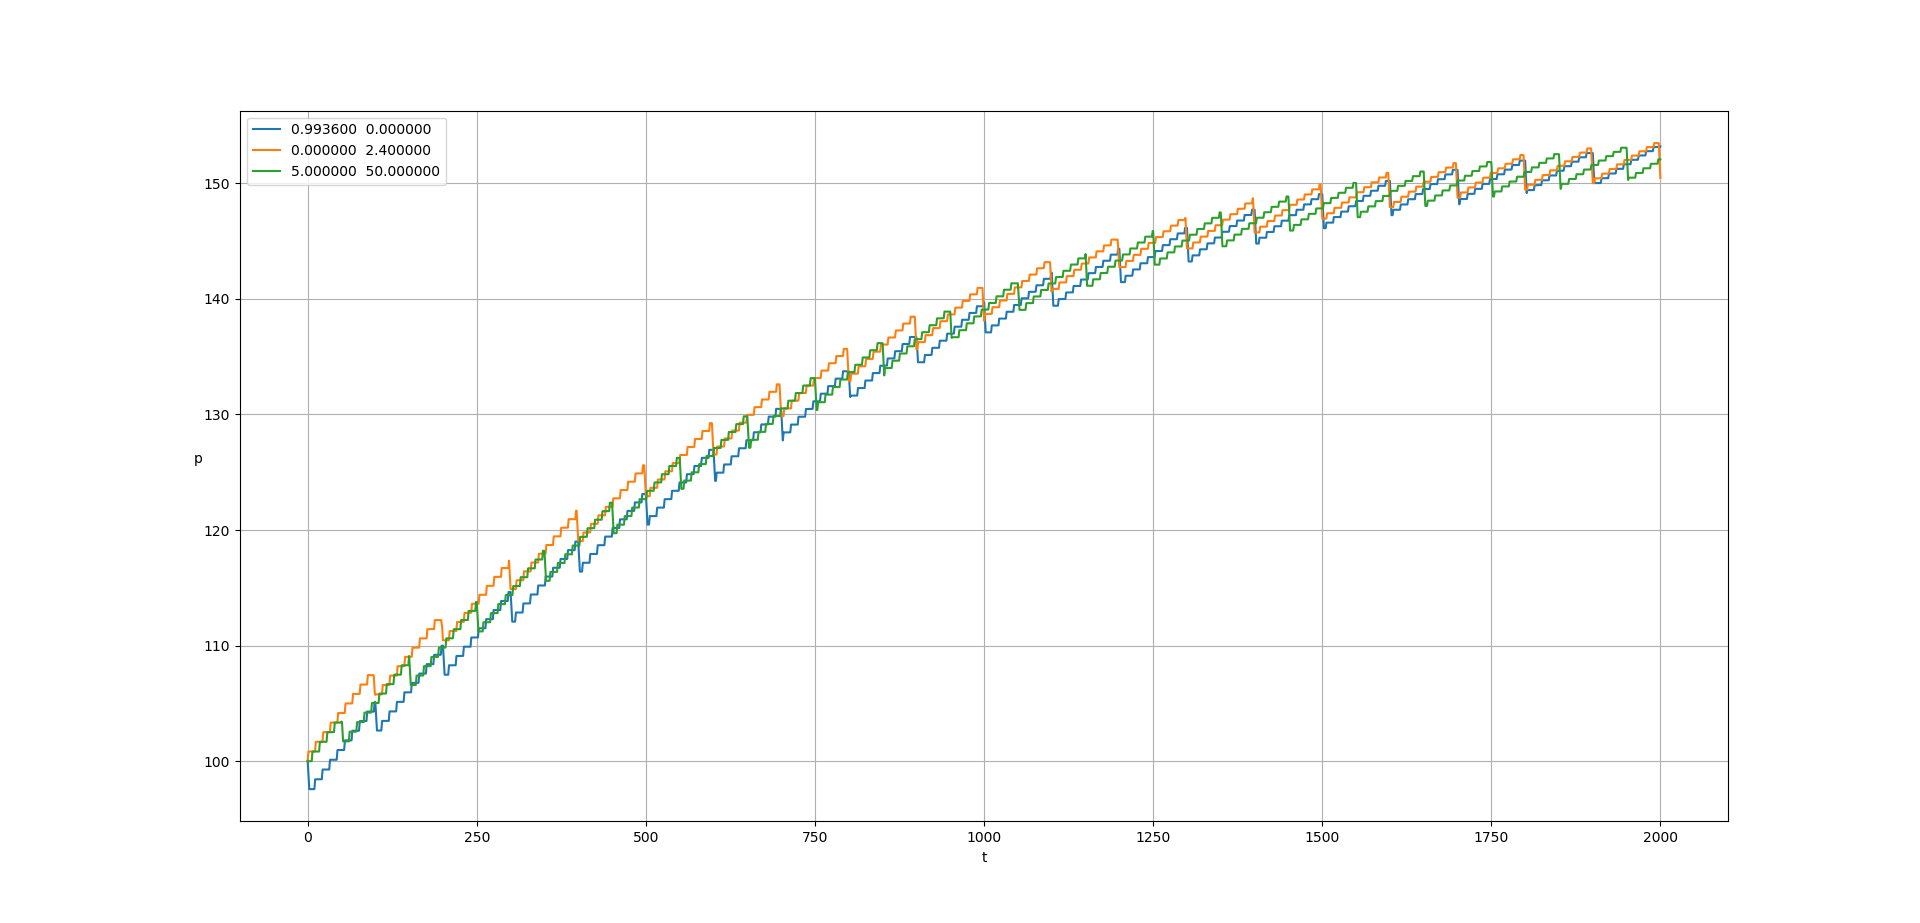
\includegraphics[scale = 0.32]{figure/12-1-exxwc.png}
        \caption{相位差对调节过程的影响}
        \label{12exxwc}
    \end{figure}
    而经过该段时间后,维持\SI{150}{\MPa}所需要的单向阀开启时长为$T_{150}=\SI{0.70}{\ms}$。图\ref{adjustpress}展示了其中一个调整过程中的压力对时间的变化图像。\par
    \paragraph{问题1结论}
    综上所述,将高压油管内的压力尽可能稳定在\SI{100}{\MPa}左右,应该设置单向阀每次开启\SI{0.29}{\ms}。如果要将高压油管内的压力从\SI{100}{\MPa}增加到\SI{150}{\MPa},且分别经过约\SI{2}{\s}、\SI{5}{\s}和\SI{10}{\s}的调整之后稳定在\SI{150}{\MPa}时的情况,对应时长内单向阀应分别先调整为开启$T_{2s}=\SI{0.89}{\ms}$、$T_{5s}=\SI{0.71}{\ms}$和$T_{10s}=\SI{0.70}{\ms}$,随后维持开启时长为$T_{150}=\SI{0.70}{\ms}$,以维持\SI{150}{\MPa}。\par
    
    \section{问题2}
    问题2中$Q_{out}(t)$的形式比较复杂。\par
    首先我们定义等效面积函数$B(t)$,用来描述针阀运动过程中喷油嘴喷孔的等效面积。由简单的几何计算可知,它的形式如下。
    \begin{equation}
        B(t)=\pi\left(\left(\frac{d_B}{2}+h(t)\tan9^\circ\right)^2-\left(\frac{d_B}{2}\right)^2\right)
    \end{equation}\par
    但是,当针阀上升到一定高度时,等效面积函数值会超过喷嘴的面积,此时喷油能力转而由喷嘴的面积限制,为了不改变$B(t)$的表达形式,我们定义了等效升程函数$h(t)$,它表示针阀的等效升程,由题目附件2给出的数据拟合,并按照前述进行修正得到,其图形和拟合结果如下
    \begin{figure}[H]
        \centering
        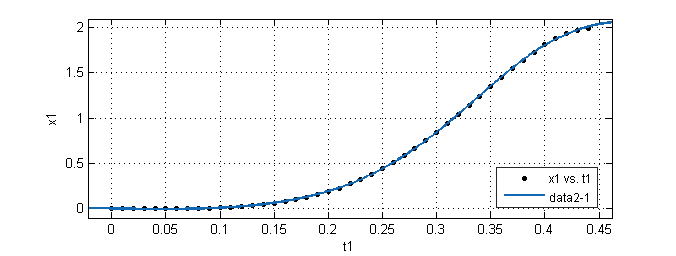
\includegraphics[scale=0.8]{figure/data21.png}
        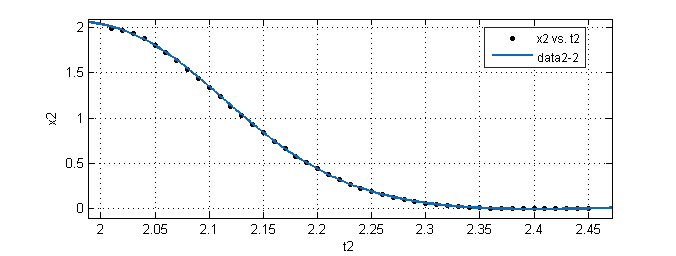
\includegraphics[scale=0.8]{figure/data22.png}
        \caption{针阀升程}
        \label{zhenfa}
    \end{figure}
    \begin{equation}
        h(t)=
        \begin{cases}
            \frac{0.5342(t-100k)^2-0.04835(t-100k)+0.000726}{(t-100k)^2-0.7362(t-100k)+0.1716}&100k\leq t\leq 100k+0.3309,k\in\mathbb{N}\\
            1.1532&100k\leq t+0.3309\leq 100k+2.1213,k\in\mathbb{N}\\
            \frac{0.5358(t-100k)^2-2.576(t-100k)+3.096}{(t-100k)^2-4.163(t-100k)+4.368}&100k+2.1213\leq t\leq 100k+2.45,k\in\mathbb{N}\\
            0&100k+2.45\leq t\leq 100(k+1),k\in\mathbb{N}\\      
        \end{cases}
    \end{equation}
    由于高压油管内的油压远高于大气压,所以我们可以忽略喷油嘴外的压强,即$\Delta p\approx p$,由此$Q_{out}(t)$就可以被写成
    \begin{equation}
        Q_{out}(t)=CB\sqrt{\frac{2p}{\rho}}
    \end{equation}\par
    再来看$Q_{in}$的表达形式,它形式上与上一题类似,如方程\ref{qin2}(以下下标为$h$的项均为油泵油缸的性质)
    \begin{equation}
        Q_{in}(t)=\delta CA\sqrt{\frac{2(p_h-p)}{\rho_h}}
        \label{qin2}
    \end{equation}
    其中$0-1$变量$\delta$定义如下
    \begin{equation}
        \delta=
        \begin{cases}
            1&p_h\geq p\\
            0&p_h<p\\
        \end{cases}
    \end{equation}\par
    下面我们来求油缸内压力$p_h$的表达式。油缸的体积可以表示为时间$t$的周期函数
    \begin{equation}
        V_h(t)=20+(R_{up}-R(\theta(t)))\pi\left(\frac{5}{2}\right)^2
    \end{equation}
    其中$R_{up}$为凸轮位于上止点时的极径,由题目给出,此时缸内压力为\SI{0.5}{\MPa},$R(\theta)$的表达式由题目附件1给出,$\theta(t)$的表达式如下,为了计算方便,我们把时刻$t=0$的相位设置为下止点,也就是$\theta = \pi$。
    \begin{equation}
        \theta(t)=\omega t+\pi -2k\pi,k\in\mathbb{N},\theta(t)\geq0
    \end{equation}
    当油泵活塞运行到下止点时,油泵吸慢了油,并不再把油返回低压油路,所以我们可以在油泵位于下止点时直接给定一个初值$p_0=\SI{0.5}{\MPa}$,对每一个周期都是这样。\par
    考虑油泵油缸的质量守恒,可以得到下面的方程。
    \begin{equation}
        \frac{\dif m_h}{\dif t}=-Q_{in}\rho
        \label{highmaineq}
    \end{equation}
    又由密度的定义$m_h=\rho_hV_h$微分得到
    \begin{equation}
        \dif m_h=\rho_h\dif V_h+V_h\dif\rho_h
        \label{higheq2}
    \end{equation}
    将方程\ref{pandrho}、\ref{highmaineq}、\ref{higheq2}联立,加入初值条件,可以整理得到
    \begin{equation}
        \begin{aligned}
            &\frac{\dif p_h}{E(p_h)\dif t}=\frac{1}{V_h}\left(-Q_{in}\frac{\rho}{\rho_h}-\frac{\dif V_h}{\dif t}\right)\\
            &p_h(\frac{2k\pi}{\omega})=0.5,k\in\mathbb{N}
        \end{aligned}
        \label{highmaineq2}
    \end{equation}\par
    在高压油泵供油的过程中我们可以用方程\ref{highmaineq2}去描述它的情况。这个方程的形式和刚才对高压油管的建模模型——方程\ref{maineq}形式很相似,也就是我们可以把高压油泵的油缸视作另一个高压油管,活塞对它的压缩可以视作$Q_{in}$,而向高压油管供油可以视作$Q_{out}$,当然此时$V$是变量,所以不可以直接代入。\par
    同时,根据方程\ref{maineq}我们可以写出高压油管的方程
    \begin{equation}
        \frac{\dif p}{E\dif t}=\frac{Q_{in}-Q_{out}}{V}
        \label{maineq2}
    \end{equation}\par
    联立方程\ref{maineq2}、\ref{highmaineq2}并使用和问题1中相似的差分方程计算
    \begin{equation}
        \begin{aligned}
            &\frac{p_{h\ i+1}-p_{h\ i}}{E(p_{h\ i})\Delta t}=\frac{1}{V_h(t_i)}\left(-\delta CA\sqrt{\frac{2\left(p_h-p_i\right)}{\rho_h}}\frac{\rho}{\rho_h}-\frac{\dif V_h}{\dif t}\right)\\
            &\frac{p_{i+1}-p_i}{E(p_i)\Delta t}=\frac{1}{V_0}\left(\delta CA\sqrt{\frac{2\left(p_h-p_i\right)}{\rho_h}}-Q_{out}(t_i)\right)\\
            &p_h(\frac{2k\pi}{\omega})=0.5,k\in\mathbb{N}
        \end{aligned}
    \end{equation}\par
    我们使用二分法对一定范围内的$\omega$进行搜索,用经过一定时间段后高压油管内油压力的变化$\Delta p$来评价“压力稳定在\SI{100}{\MPa}”的好坏,搜索出使压力变化最小时的$\omega=\SI{0.027}{\radian\per\ms}$。对应的$p-t$变化曲线如图\ref{ptfigure2}。\par
    \begin{figure}[h]
        \centering
        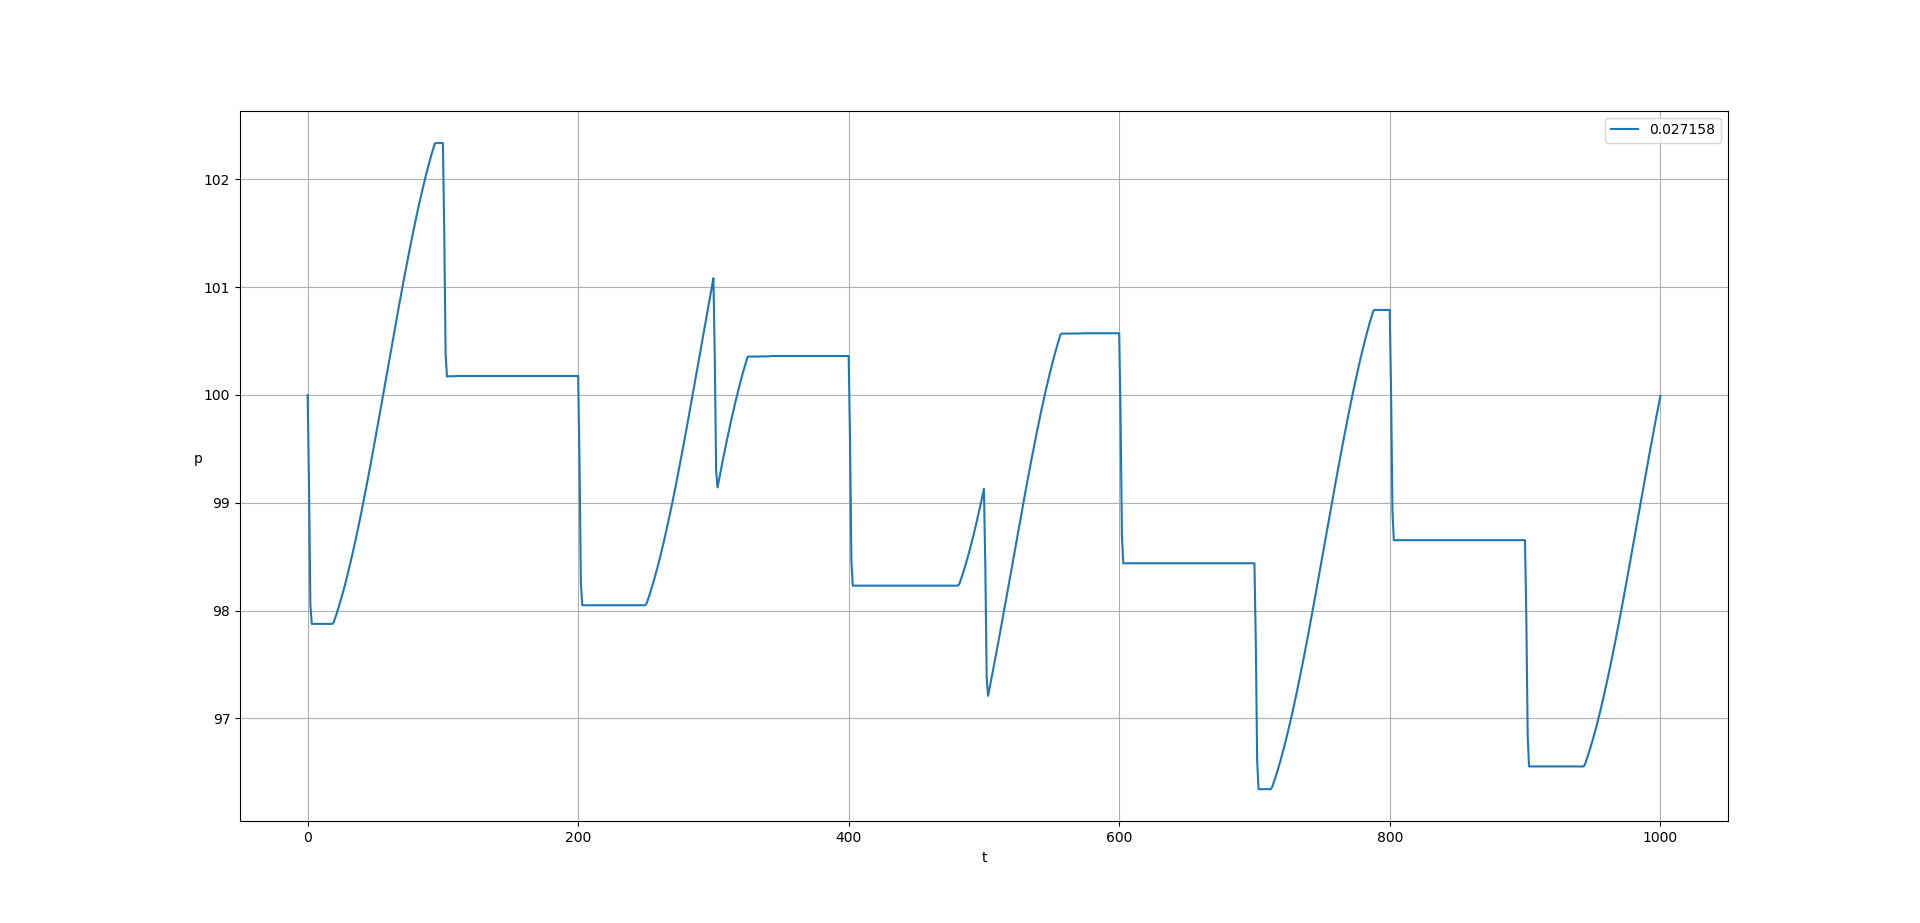
\includegraphics[scale = 0.32]{figure/2-1.png}
        \caption{问题2中高压油管内压力和时间的变化图}
        \label{ptfigure2}
    \end{figure}
    下面的曲线则描述了二分搜索中不同$\omega$的选取造成的$p-t$变化曲线。
    \begin{figure}[H]
        \centering
        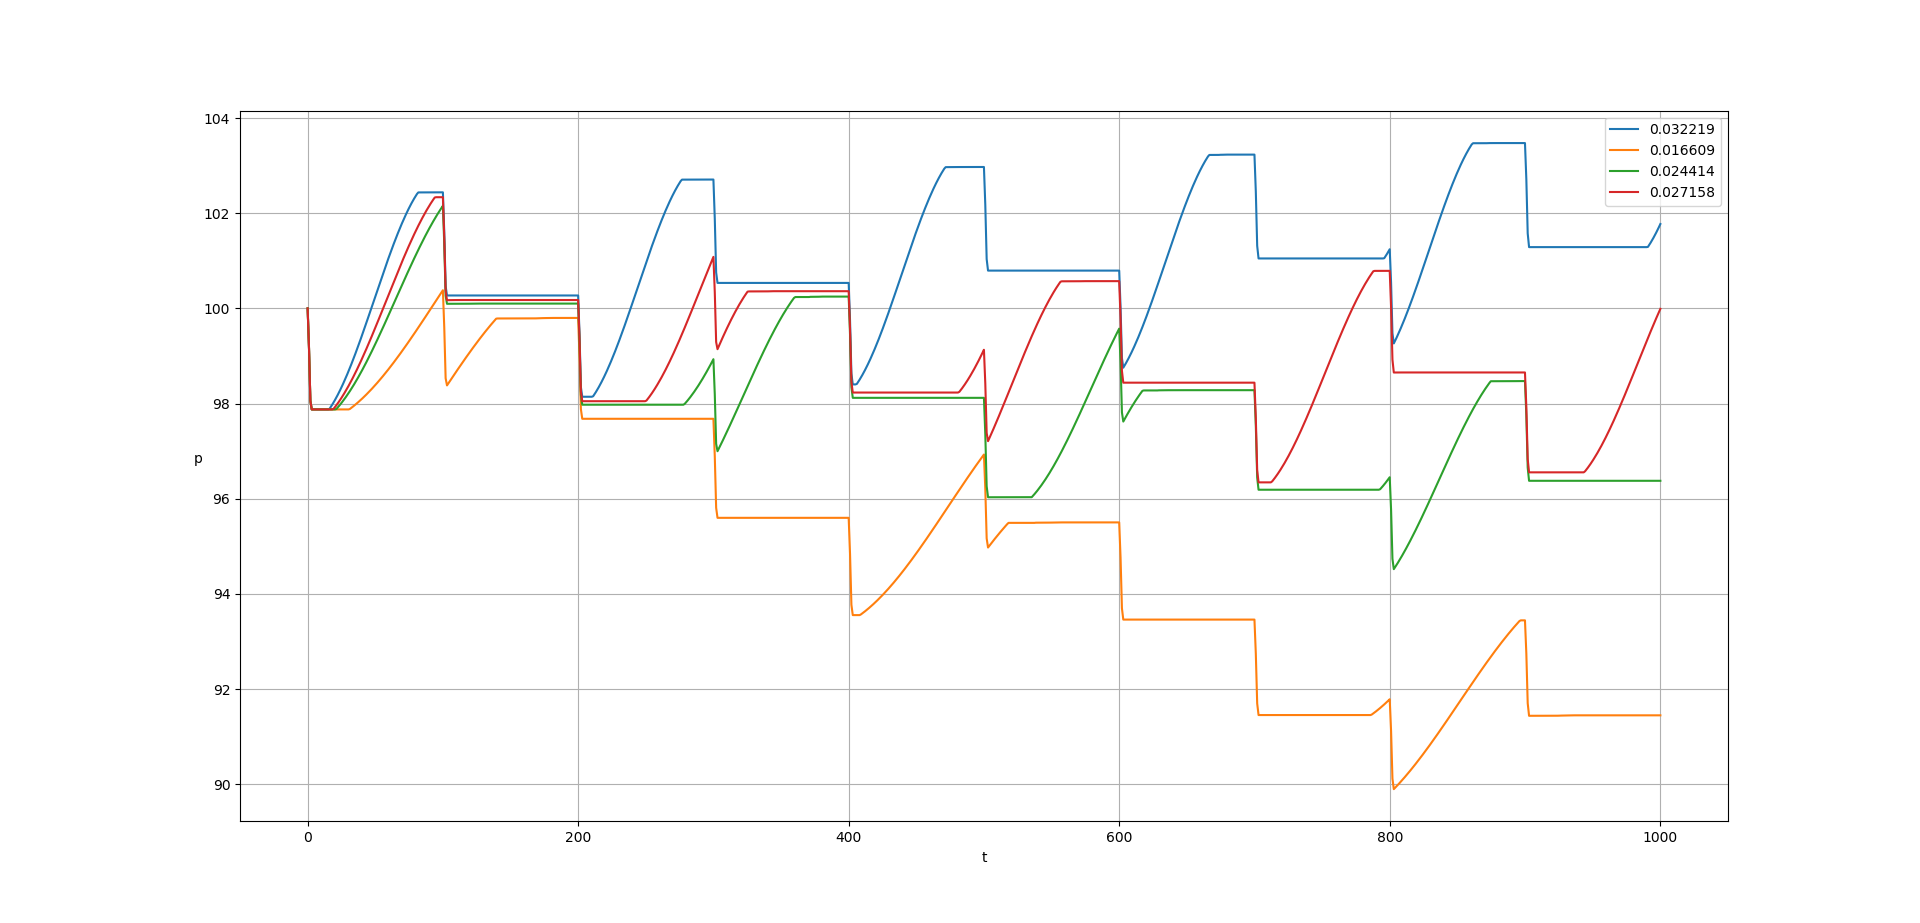
\includegraphics[scale=0.32]{figure/3-2.png}
        \caption{二分搜索中不同$\omega$的选取造成的$p-t$变化}
        % \label{}
    \end{figure}
    \paragraph{问题2结论}
    通过数值模拟和二分搜索,我们给出凸轮的角速度$\omega=\SI{0.027}{\radian\per\ms}$时,高压油管内的压力尽量稳定在\SI{100}{\MPa}左右。
    \section{问题3}
    从问题2给出的图\ref{ptfigure2}可以看到,造成压力波动的主要因素是喷油和注油过程。相比两个喷油嘴同时喷油,交替喷油可以减少高压油管中的压力波动。我们可以通过数值模拟验证这一点。\par
    增加一个喷油嘴只改变了问题2中$Q_{out}(t)$的具体形式,对于交替喷油模型,$Q_{out}(t)$的具体形式如下。\par
    \begin{equation}
        Q_{out}(t)=CB\sqrt{\frac{2p}{\rho}}
    \end{equation}
    \begin{equation}
        B(t)=\pi\left(\left(\frac{d_B}{2}+h(t)\tan9^\circ\right)^2-\left(\frac{d_B}{2}\right)^2\right)
    \end{equation}
    \begin{equation}
        h(t)=
        \begin{cases}
            \frac{0.5342(t-50k)^2-0.04835(t-50k)+0.000726}{(t-50k)^2-0.7362(t-50k)+0.1716}&50k\leq t\leq 50k+0.3309,k\in\mathbb{N}\\
            1.1532&50k\leq t+0.3309\leq 50k+2.1213,k\in\mathbb{N}\\
            \frac{0.5358(t-50k)^2-2.576(t-50k)+3.096}{(t-50k)^2-4.163(t-50k)+4.368}&50k+2.1213\leq t\leq 50k+2.45,k\in\mathbb{N}\\
            0&50k+2.45\leq t\leq 50(k+1),k\in\mathbb{N}\\      
        \end{cases}
    \end{equation}
    将这个结果代回方程\ref{maineq2}就可以进行与问题1相同的数值模拟,解出此时最合适的凸轮角速度为$\omega=\SI{0.053}{\radian\per\ms}$。图\ref{ptfigure31}中的红色线描述了此时的$p-t$变化情况,其他色线描述了二分逼近的结果。\par
    \begin{figure}[H]
        \centering
        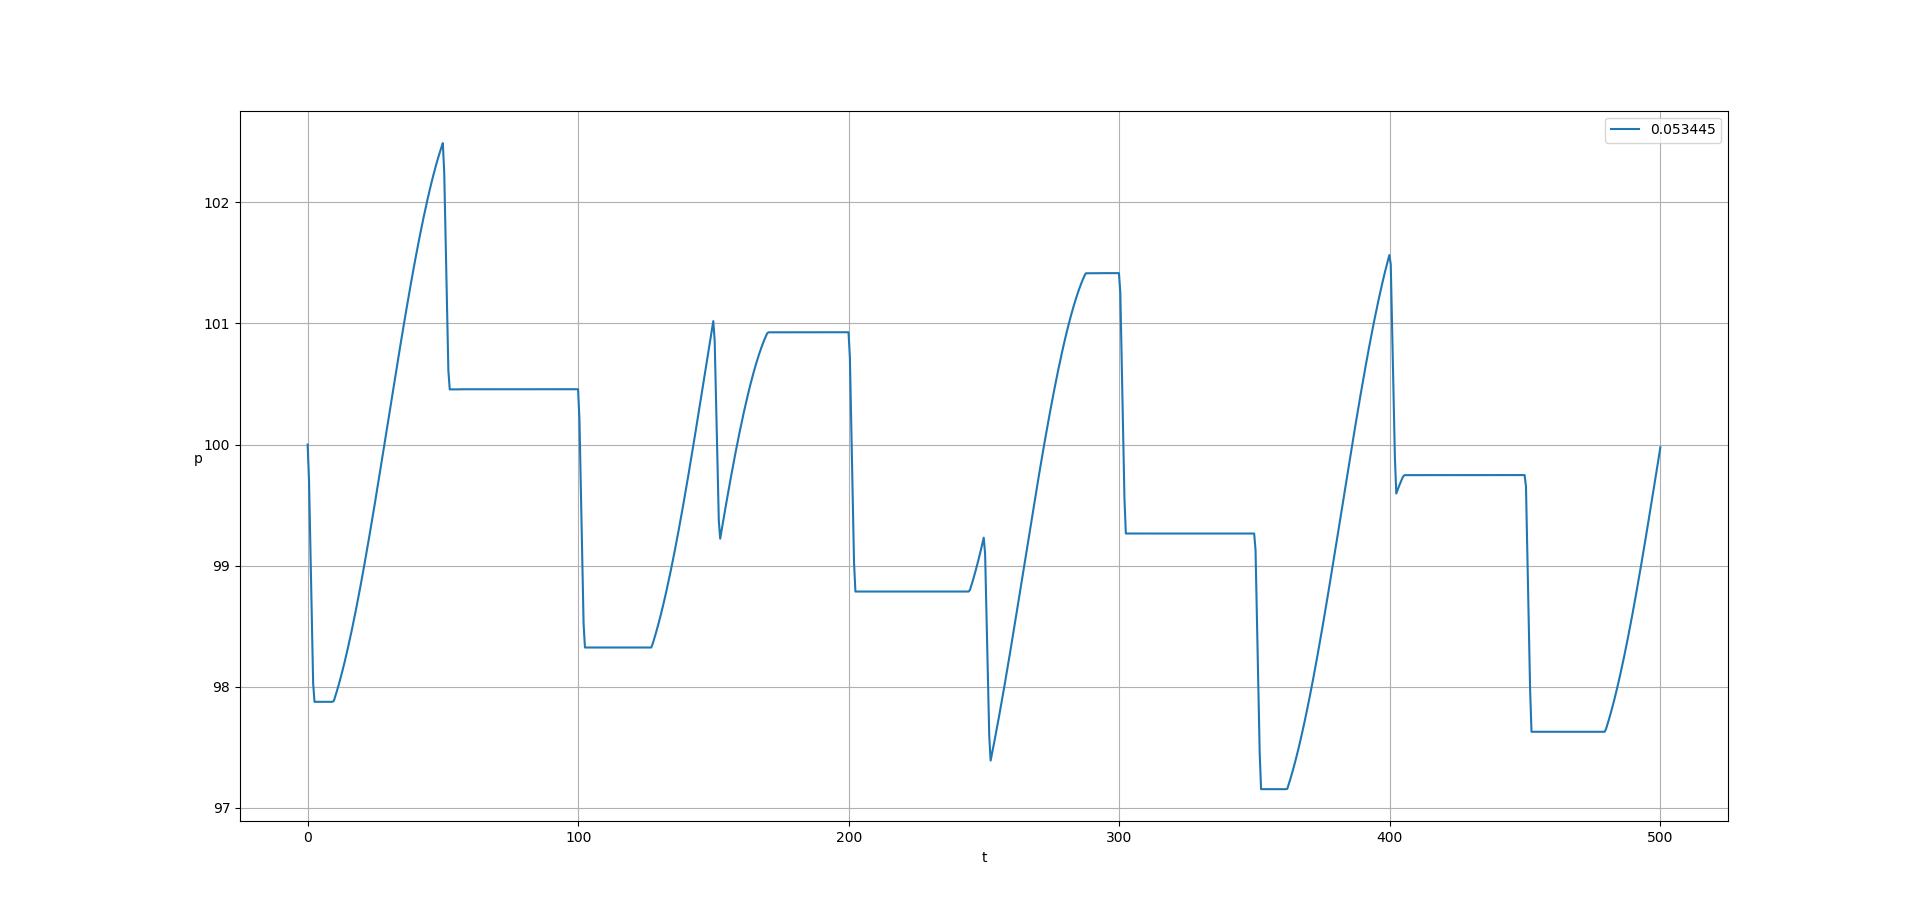
\includegraphics[scale=0.32]{figure/3-4.png}
        \caption{增加一个喷油嘴之后的高压油管内压力与时间变化}
        \label{ptfigure31}
    \end{figure}
    减压阀可以控制体系内部压力不高于某一定值,该定值即为减压阀的开放阈值,记作$p_0$,通过设定$p_0$即可控制减压阀,减压阀可以视为一个受压力控制的的喷油嘴,其对$Q_{out}(t)$的贡献为
    \begin{equation}
        Q_{out}(t)=\gamma CA\sqrt{\frac{2p}{\rho}}
    \end{equation}
    其中$0-1$变量$\gamma$定义如下
    \begin{equation}
        \gamma=
        \begin{cases}
            1&p\geq p_0\\
            0&p<p_0
        \end{cases}
    \end{equation}\par
    由于减压阀的流量亦受到流量公式的限制,所以我们不妨设定$p_0=\SI{100}{\MPa}$,并在这一条件下用经过足够长的时间后的压力变化$\Delta p$来衡量“控制高压油管压力”的好坏,利用二分搜索使$\Delta p$最小的油泵转速$\omega$的值,数值模拟得到的图如下。
    \begin{figure}[H]
        \centering
        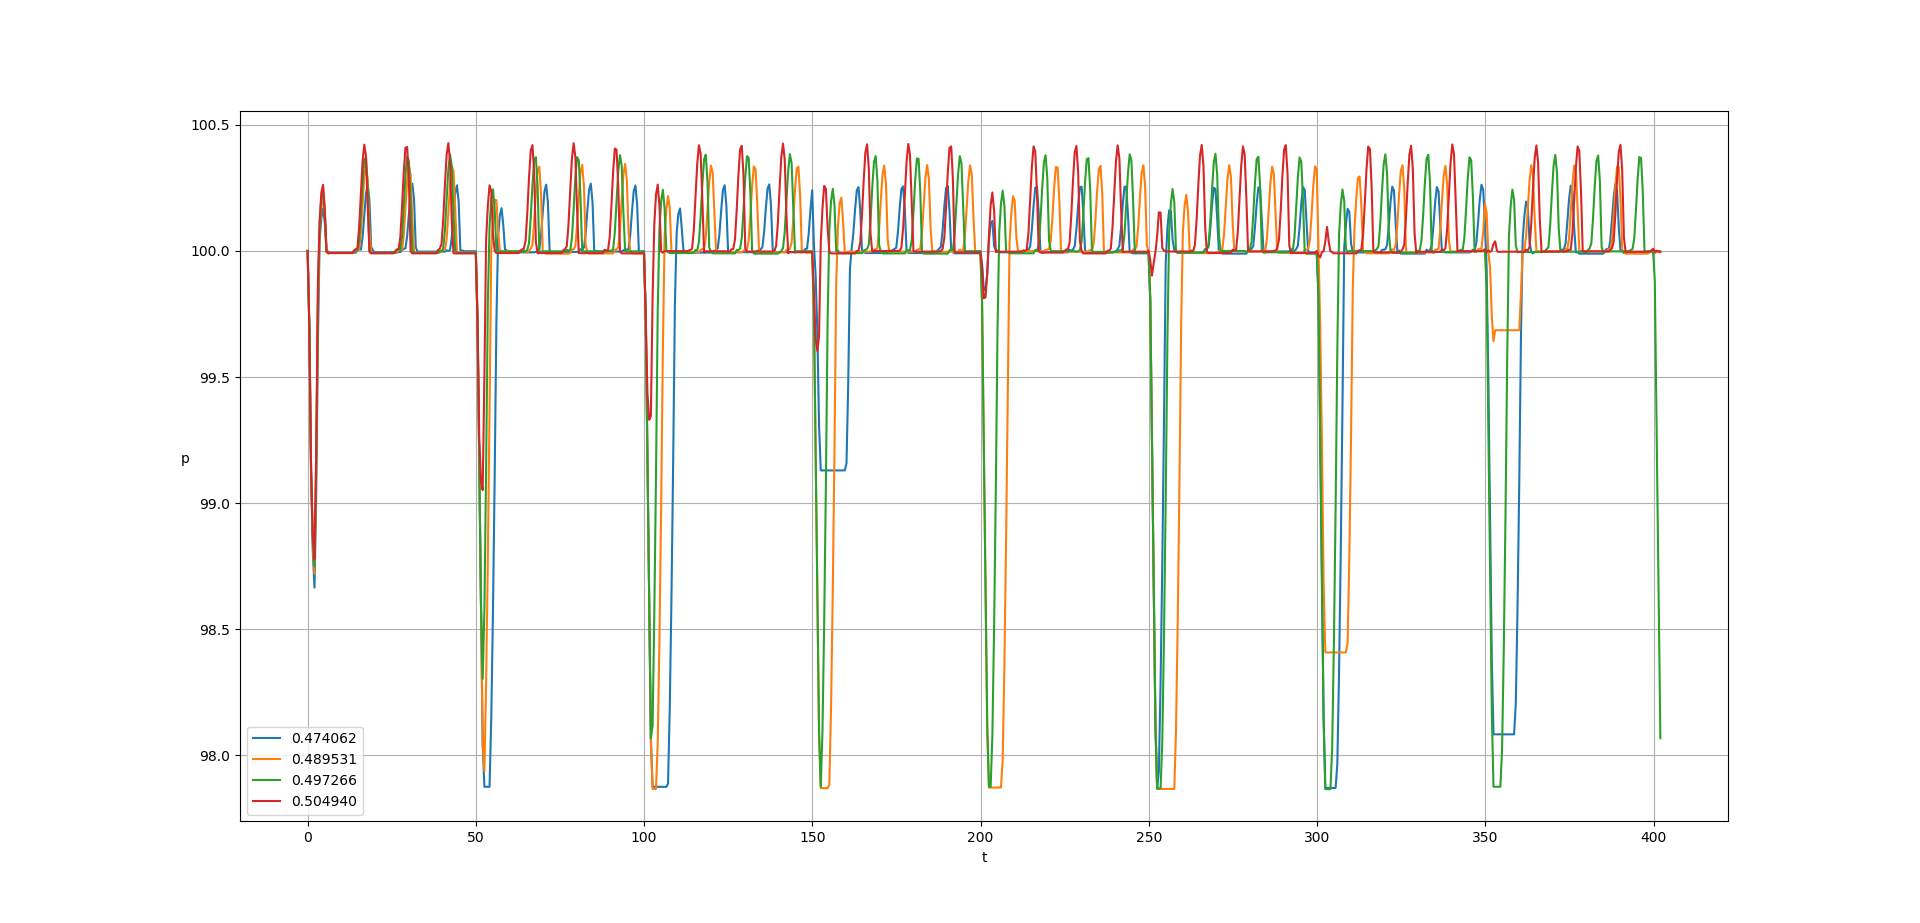
\includegraphics[scale=0.32]{figure/3-5.png}
        \caption{不同转速$\omega$对高压油管压力对时间关系的影响}
        % \label{}
    \end{figure}\par
    数值模拟结果显示,当$\omega=\SI{0.505}{\radian\per\ms}$时,$\Delta p$值最小,且压力波动范围已经显著小于原先不加减压阀的情况,所以我们选择这种方案。
    \paragraph{问题3结论}
    在增加一个喷嘴的情况下,最佳方案是使两个喷嘴交替喷油,每次喷油时间间隔相等,此时油泵转速设定为\SI{0.053}{\radian\per\ms}。加入减压阀后,控制方案为设定减压阀的打开阈值为$p_0=\SI{100}{\MPa}$,此时油泵转速对应设定为\SI{0.505}{\radian\per\ms}。

    
    \section{总结}
    在本题中,我们从简单到复杂考虑了高压油路系统的三种模型,并把它们统一到
    \[\frac{\dif p}{E\dif t}=\frac{Q_{in}-Q_{out}}{V}\]
    这一简洁的形式,利用具体条件下不同$Q_{in}$和$Q_{out}$的形式代入方程,将微分方程离散化为差分方程,利用计算机模拟求解,将优化目标量化为$\Delta p$这样的函数,并用二分法高效取得我们需要优化的值。\par

    % appendix
    \newpage
    \pagestyle{empty}
    \section{附录}
    我们使用的软件与工具包括MATLAB、Python、C++、\LaTeX、git、github和cnki.net。
    \subsection{MATLAB代码}
    我们使用MATLAB进行拟合运算,没有输入交互代码,只用鼠标操作。
    \subsection{Python代码}
    我们使用Python绘制本文中几乎大多数插图,使用的程序代码如下
    \begin{lstlisting}[language={python}]
    import matplotlib.pyplot as plt
    f=open('data.out')
    r=f.read()
    r=r.split('\n\n')
    r.pop()
    x=[];y=[]
    for i in range(len(r)):
        x.append([]);y.append([])
        r[i]=r[i].split('\n')
        for j in range(len(r[i])-1):
            r[i][j]=r[i][j].split(' ')
            x[i].append(float(r[i][j][0]))
            y[i].append(float(r[i][j][1]))
        plt.plot(x[i],y[i],label=str(r[i][len(r[i])-1]))
        print(str(r[i][len(r[i])-1]))
    plt.xlabel('t');plt.ylabel('p',rotation=0)
    plt.legend()
    plt.grid()
    plt.show()
    \end{lstlisting}
    \subsection{C++代码}
    本题中所有的二分法优化都是通过不断改动以下程序的参数实现的
    \begin{lstlisting}[language={c++}]
    #include<cstdio>
    #include<cmath>
    #define TimeLimit 1000
    #define GAP 0.01
    #define INIT 100
    #define V (3.1416*500*25)
    #define C 0.85
    #define Phigh 160
    #define Precision 0.001
    #define DIF 0
    #define phinit 0.5
    double omege = 20;
    // #define INF 
    /*//this part for question 1
    double T = 0.3;
    double A(double t)
    {
        double temp = t-(double)((int)(t/(T+10)))*(T+10);
        if(temp <= T){
            return (0.49*3.1416);
        }
        else return 0;
    }
    double Qout(double t)
    {
        double temp = t-(double)((int)(t/(100)))*(100);
        // printf("%f",temp);
        if(temp <= 0.2)
        {
            return 100*temp;
        }
        else if(temp >0.2 && temp < 2.2)
        {
            return 20;
        }
        else if(temp >= 2.2 && temp <= 2.4)
        {
            return temp*(-100)+240;
        }
        else return 0;
    }
    double p()
    {
        double t = 0;
        double press = INIT;
        // printf("%f\n%f\n",t,press);
        while (t < TimeLimit)
        {
            // printf("press=%f\t",press);
            if(press > Phigh)press = Phigh;
            press = press + ((C*A(t)*sqrt(2*(Phigh-
            press)/0.87113)-Qout(t))/V)*GAP
            *(0.0001*press*press*press-0.001082
            *press*press+5.474*press+1532);
            t += GAP;
            // printf("%f\n%f\n",t,press);
        }
        return (press - INIT);
    }
    */
    double rho(double p){
        double sum=0;
        if(p>100){
            for(double i=100;i<=p;i+=0.001){
                sum+=0.001/(0.0001*i*i*i-0.001082*i
                *i+5.474*i+1532);
            }
            return 0.85*pow(2.718281828459,sum);
        }
        else if(p<100){
            for(double i=100;i>=p;i-=0.001){
                sum-=0.001/(0.0001*i*i*i-0.001082*i
                *i+5.474*i+1532);
            }
            return 0.85*pow(2.718281828459,sum);
        }
        return 0.85;
    }
    inline double E(double p)
    {
        return (0.0001*p*p*p-0.001082*p*p+5.474*p
        +1532);
    }
    inline int delta(double ph, double p)
    {
        return (ph >= p);
    }
    inline double Theta(double t)
    {
        return (omege*t+3.14-6.28*(int)((omege*t
        +3.14)/6.28));
    }
    inline double R(double theta)
    {
        return (4.826+2.413*sin(theta+1.5708));
    }
    double Vh(double t)
    {
        return (20+(7.239-R(Theta(t)))*3.1416*2.5
        *2.5);
    }
    double h(double t)
    {
        double temp = t - ((int)(t/50))*50;
        if(temp < 0.3309)
        {
            return (0.5342*temp*temp-0.04835*temp+
            0.000726)/(temp*temp-0.7362*temp+0.1716);
        }
        else if(temp >= 0.3309 && temp <= 2.1213)
        {
            return 1.1532;
        }
        else if(temp > 2.1213 && temp < 2.45)
        {
            return (0.5358*temp*temp-2.576*temp+
            3.096)/(temp*temp-4.163*temp+4.368);
        }
        else
        {
            return 0;
        }
    }
    double B(double t)
    {
        return 3.1416*((1.25+h(t)*0.1584)*(1.25
        +h(t)*0.1584)-1.25*1.25);
    }
    double Qout(double t, double p)
    {
        return (0.85*B(t)*sqrt(2*p/rho(p)));
    }
    double p()//for question 2
    {
        double t = 0;
        double press = INIT;
        double pressh = phinit;
        // printf("%f\n%f\n",t,press);
        while (t < TimeLimit)
        {
            // printf("press=%f\t",press);
            t += GAP;
            if(omege*t/6.2832-(int)(omege*t
            /6.2832) < 0.001 && omege*t/6.2832
            -(int)(omege*t/6.2832) > -0.001)
            {
                pressh = phinit;
            }
            // printf("Qout = %f\t",
            Qout(t,press));//喷油
            if(delta(pressh,press))
            {
                // printf("inittime = %f\tpressh
                = %f\tpress = %f\n",t,pressh,press);
                pressh = pressh + (GAP*E(pressh)
                /Vh(t))*(-0.85*3.1416*0.49*sqrt(2
                *(pressh - press)/rho(pressh))
                *(rho(press)/rho(pressh)) - (Vh(t)
                 - Vh(t - GAP))/GAP);
                if(delta(pressh,press))
                {
                    press = press + (GAP*E(press)/V)
                    *(0.85*3.1416*0.49*sqrt(2*(pressh
                     - press)/rho(pressh)) - Qout(t
                     ,press));        
                }
                else
                {
                    press = press + (GAP*E(press)/V)
                    *( - Qout(t,press));
                }    
            }
            else
            {
                pressh = pressh + (GAP*E(pressh)
                /Vh(t))*( - (Vh(t) - Vh(t - GAP))/GAP);
                press = press + (GAP*E(press)/V)
                *( - Qout(t,press));
            }
            // printf("time = %f\tpressh = %f\tpress
             = %f\n",t,pressh,press);
        }
        return (press - INIT);
    }
    void binarysearch(double start, double end)
    {
        printf("search[%f,%f]\t",start,end);
        if (end - start < Precision)
        {
                printf("found the solution : %f",end);
            return;
        }
        omege = start + (end - start)/2;
        double mid = p();
        printf("mid p=%f\n",mid);
        if(mid - DIF > 0){
            binarysearch(start, start + (end - start)/2);
        }
        else
        {
            binarysearch(start + (end - start)/2, end);
        }
    }
    int main()
    {
        
        // freopen("dataof1.out","w",stdout);
        // printf("%f",(GAP*E(102)/V)*( - Qout(57,102)) );
        binarysearch(0.03,0.1);
    
        return 0;
    }
    \end{lstlisting}
    \subsection{\LaTeX 代码}
    本文用\LaTeX 排版,\LaTeX 代码置于支持文件中。

\end{document}